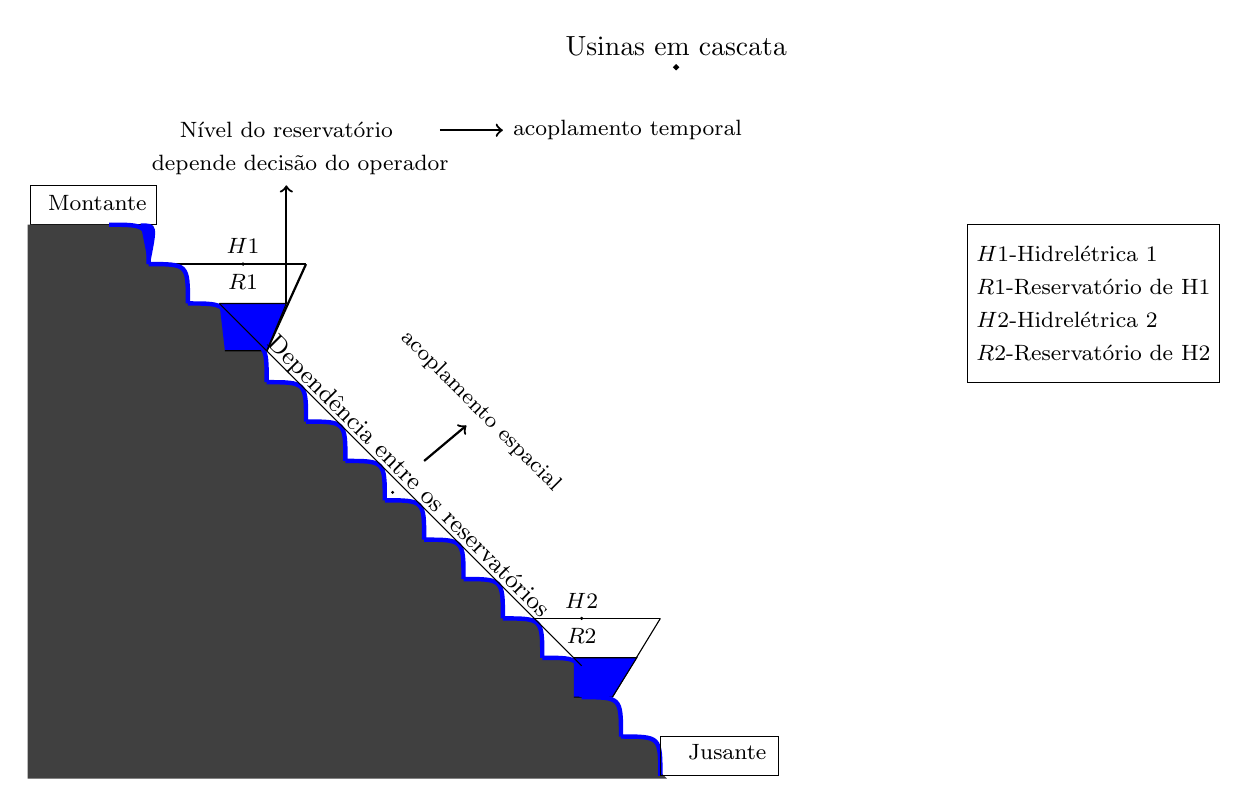
\begin{tikzpicture}
  % Desenho da cascata
  \draw [ultra thick,black] (7.2,9.0) circle (0.01mm) node[above]{Usinas em cascata};
  %
  % Desenho da montante
  \draw (-1.0,7.0) rectangle (0.6, 7.5) 
  node[below left] {\footnotesize Montante};
  %
  % Desenho da jusante

  \draw [thick, black]  (-1,0)--(-1,7);
  \draw [thick, black]  (-1,0)--(7,0);
  \draw [fill=darkgray] (-1.0,7.0) .. controls (0.5,7.0) .. (0.5,6.5);
  \draw [fill=darkgray] (0.0,7.0) .. controls (0.5,7.0) .. (0.5,6.5);
  \draw [fill=darkgray] (0.5,6.5) .. controls (1.0,6.5) .. (1.0,6.0);
  \draw [fill=darkgray] (1.0,6.0) .. controls (1.5,6.0) .. (1.5,5.5);
  \draw [fill=darkgray] (1.5,5.5) .. controls (2.0,5.5) .. (2.0,5.0);
  \draw [fill=darkgray] (2.0,5.0) .. controls (2.5,5.0) .. (2.5,4.5);
  \draw [fill=darkgray] (2.5,4.5) .. controls (3.0,4.5) .. (3.0,4.0);
  \draw [fill=darkgray] (3.0,4.0) .. controls (3.5,4.0) .. (3.5,3.5);
  \draw [fill=darkgray] (3.5,3.5) .. controls (4.0,3.5) .. (4.0,3.0);
  \draw [fill=darkgray] (4.0,3.0) .. controls (4.5,3.0) .. (4.5,2.5);
  \draw [fill=darkgray] (4.5,2.5) .. controls (5.0,2.5) .. (5.0,2.0);
  \draw [fill=darkgray] (5.0,2.0) .. controls (5.5,2.0) .. (5.5,1.5);
  \draw [fill=darkgray] (5.5,1.5) .. controls (6.0,1.5) .. (6.0,1.0);
  \draw [fill=darkgray] (6.0,1.0) .. controls (6.5,1.0) .. (6.5,0.5);
  \draw [fill=darkgray] (6.5,0.5) .. controls (7.0,0.5) .. (7.0,0.0);
  \draw [fill=darkgray,line width=0.1pt, opacity=100] (0,7)--(7,0);
  \filldraw [darkgray, line width=2.0pt] (0,7)--(7,0)--(-1,0)--(-1,7);
  %
  % Desenho de H1 
  \draw [thick, black] (1.7,6.5) circle (0.01mm) node [above]{\footnotesize $H1$};
  \draw [thick, black] (0.5,6.5)--(2.5,6.5);
  \draw [thick, black] (1.7,6.5) circle (0.01mm) node [below]{\footnotesize $R1$};
  \draw [thick, black] (2.5,6.5)--(2.0,5.4);
  
  \draw [fill=blue](1.40,6.0)--(2.25,6.0)--(2.0,5.4)--(1.47,5.4);
  % 
  % Desenho de H2
  \draw [thick, black] (6.0, 2.0) circle (0.01mm) node[above]{ \footnotesize $H2$};
  \draw [fill=darkgray] (5.0,2.0) -- (7.0,2.0);
  \draw [thick, black] (6.0,2.0) circle (0.01mm) node [below]{\footnotesize $R2$};
  \draw [fill=darkgray] (7.0,2.0) -- (6.39,1.0);
  \draw [fill=blue] (5.9,1.5) -- (6.7,1.5) --(6.39,1.0) -- (5.9, 1.0); 
  %
  % Desenho fio de agua
  \filldraw [blue, line width=1pt] (0.4, 7.0) .. controls (0.6, 7.0) .. (0.5,6.5);

  \draw [blue, ultra thick] (0.0,7.0) .. controls (0.5,7.0) .. (0.5,6.5);
  \draw [blue, ultra thick] (0.5,6.5) .. controls (1.0,6.5) .. (1.0,6.0);
  \draw [blue, ultra thick] (1.0,6.0) .. controls (1.5,6.0) .. (1.5,5.5);
  \draw [blue, ultra thick] (1.5,5.5) .. controls (2.0,5.5) .. (2.0,5.0);
  \draw [blue, ultra thick] (2.0,5.0) .. controls (2.5,5.0) .. (2.5,4.5);
  \draw [blue, ultra thick] (2.5,4.5) .. controls (3.0,4.5) .. (3.0,4.0);
  \draw [blue, ultra thick] (3.0,4.0) .. controls (3.5,4.0) .. (3.5,3.5);
  \draw [blue, ultra thick] (3.5,3.5) .. controls (4.0,3.5) .. (4.0,3.0);
  \draw [blue, ultra thick] (4.0,3.0) .. controls (4.5,3.0) .. (4.5,2.5);
  \draw [blue, ultra thick] (4.5,2.5) .. controls (5.0,2.5) .. (5.0,2.0);
  \draw [blue, ultra thick] (5.0,2.0) .. controls (5.5,2.0) .. (5.5,1.5);
  \draw [blue, ultra thick] (5.5,1.5) .. controls (6.0,1.5) .. (6.0,1.0);
  \draw [blue, ultra thick] (6.0,1.0) .. controls (6.5,1.0) .. (6.5,0.5);
  \draw [blue, ultra thick] (6.5,0.5) .. controls (7.0,0.5) .. (7.0,0.0);
  %
  % Desenho da legenda
   \node [draw,align=justify, minimum size=2cm]() at (12.5,6.0) {\footnotesize $H1$-\footnotesize Hidrel\'etrica 1 \\
  \footnotesize $R1$-\footnotesize Reservat\'orio de H1 \\ 
  \footnotesize $H2$-\footnotesize Hidrel\'etrica 2 \\
  \footnotesize $R2$-\footnotesize Reservat\'orio de H2};
  %\draw (9.5,4.5) rectangle (13.5,7.0); 
  %\draw (11.0,6.5) circle (0.01mm) node[] {\footnotesize $H1$-\footnotesize Hidrel\'etrica 1};
  %\draw (11.3,6.0) circle (0.01mm) node[] {\footnotesize $R1$-\footnotesize Reservat\'orio de H1};
  %\draw (11.0,5.5) circle (0.01mm) node[] {\footnotesize $H2$-\footnotesize Hidrel\'etrica 2};
  %\draw (11.3,5.0) circle (0.01mm) node[] {\footnotesize $R2$-\footnotesize Reservat\'orio de H2};
  %
  % Desenho do acoplamento temporal
  \draw (1.4,6)--(6,1.4);
  \draw [thick, black] (3.6,3.6) circle (0.01mm) node[above, rotate=315]{\fontsize{9}{12}\selectfont {Depend\^encia entre os
  reservat\'orios}};
  \draw [->,thick, black,rotate around={-50:(4.0,4.0)}]
	(4.0,4.0)--(4.0,4.7)node[above, rotate=315]{\footnotesize acoplamento espacial};
	\draw [->,thick, black](2.25,6.0)--(2.25,7.5) node[above,align=center]{\footnotesize N\'ivel do reservat\'orio 
	\\ \quad \footnotesize depende decis\~ao do operador};
	\draw [->,thick, black] (4.2,8.2) -- (5.0,8.2) node[right] {\footnotesize acoplamento temporal};
	%
	% Desenho da Jusante
	\draw (7.0,0.0) rectangle (8.5, 0.5);
	\draw (7.8,0.3) circle (0.01mm) node[]{\footnotesize{} Jusante};  
\end{tikzpicture}
